\chapter{Réalisation}\label{realisation}

\section{Capture d'images}\label{realisation.capture}
\subsection{Emplacement de la caméra}
En date du 29 mai 2018, la caméra a été installée, connectée au réseau et est fonctionnelle. La photo présentée en figure \ref{fig:cam_parking_annotation} est une vue aérienne du site de Cheseaux de la HEIG-VD. C'est ici qu'un parking sera filmé.

\begin{figure}[H]
    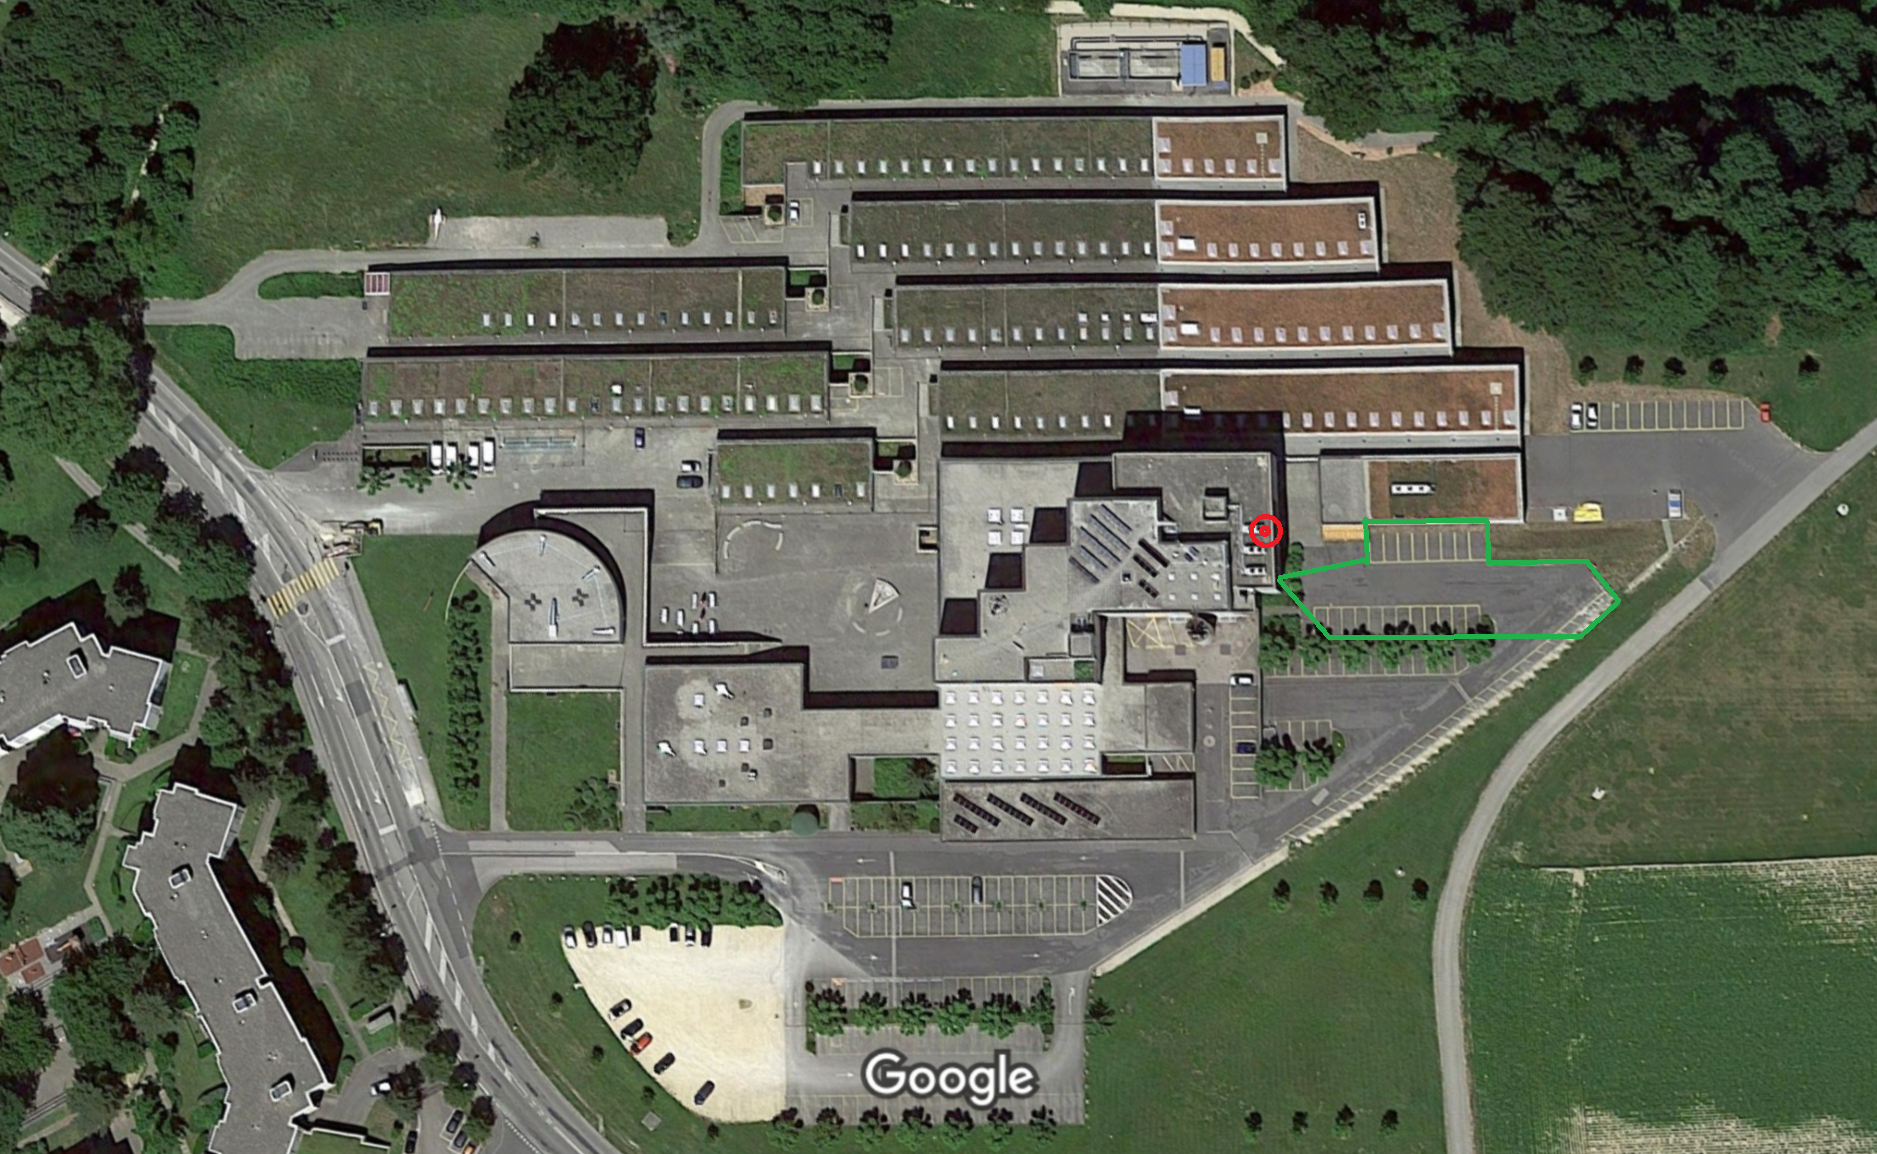
\includegraphics[width=14cm]{img/conception/cam_parking_location.png}
    \centering
    \captionsource{Emplacement de la caméra (en rouge) et du parking filmé (en vert)}{map:heig-vd}
    \label{fig:cam_parking_annotation}
\end{figure} 

Y est désigné par un cercle rouge l'emplacement de la caméra. Elle se situe sur la terrasse du bâtiment est, accessible au niveau K. Elle est orientée afin de pouvoir capturer des images du parking désigné en vert. 

Malheureusement, lors des tests effectués après réception de la caméra \textbf{Wanscam} \textit{HW0029-5}, il a été remarqué que le signal Wifi présent sur le toit n'était pas suffisamment fiable afin de connecter la caméra. Afin de palier à ce problème, un câble réseau Ethernet a tout de même pu être tiré de manière temporaire.

\subsection{Configuration des périphériques}
Dans cette sous-section, on trouvera des informations utiles concernant la caméra et la machine virtuelle. Ces informations seront utilisées dans la suite de ce rapport. 

Afin de pouvoir accéder à la caméra, un FQDN\footnote{\textit{FQDN}: \textit{Fully qualified domain name}, soit nom de domaine entièrement qualifié. \autocite{wiki:FQDN}} a été configuré. Celui-ci permet d'obtenir l'adresse IP de la caméra à l'aide du DNS local. Ainsi, plutôt que de s'adresser à elle par une adresse IP, il suffit d'utiliser en lieu et place l'adresse suivante:
\begin{center}
    \textit{ipcam.einet.ad.eivd.ch}
\end{center}

%\nomenclature{FQDN}{\textit{Fully qualified domain name}, soit nom de domaine entièrement qualifié}

Comme indiqué en section \ref{conception.architecture.capture.logique}, une VM est mise à disposition de ce projet afin de récupérer des images de la caméra. Son adresse IP, 10.192.75.100, est fixe.

\subsection{Requêtes et protocole}
La caméra \textbf{Wanscam} \textit{HW0029-5} expose un serveur web permettant sa configuration. Bien entendu, celui-ci permet des connexions authentifiées. Il utilise le protocole \textit{Basic Auth HTTP\footnote{Le protocole Basic Auth consiste à inclure dans les entêtes HTTP un champ \textit{Authorization}. Celui-ci contient le login et le mot de passe de l'utilisateur, sous forme encodée (\textit{Base64})}}\autocite{wiki:basic-auth}. Il est cependant important de remarquer que le serveur ne permet pas l'utilisation d'\textit{HTTPS}: ainsi, la connexion n'est pas chiffrée. Le mot de passe fournit à la caméra, bien qu'encodé, circule en clair sur le réseau. Il est  donc important de noter que dans le cadre d'une application professionnelle, ceci n'est pas envisageable.

Elle expose un \textit{endpoint} \textit{HTTP} permettant de récupérer l'image actuelle que filme la caméra. Ainsi, dans le cadre de ce projet, l'adresse \textit{http://ipcam.einet.ad.eivd.ch/web/tmpfs/snap.jpg} est utilisée. La figure \ref{fig:image_request} présente donc ce protocole de communication qui est utilisé afin de récupérer des images.

\begin{figure}[H]
    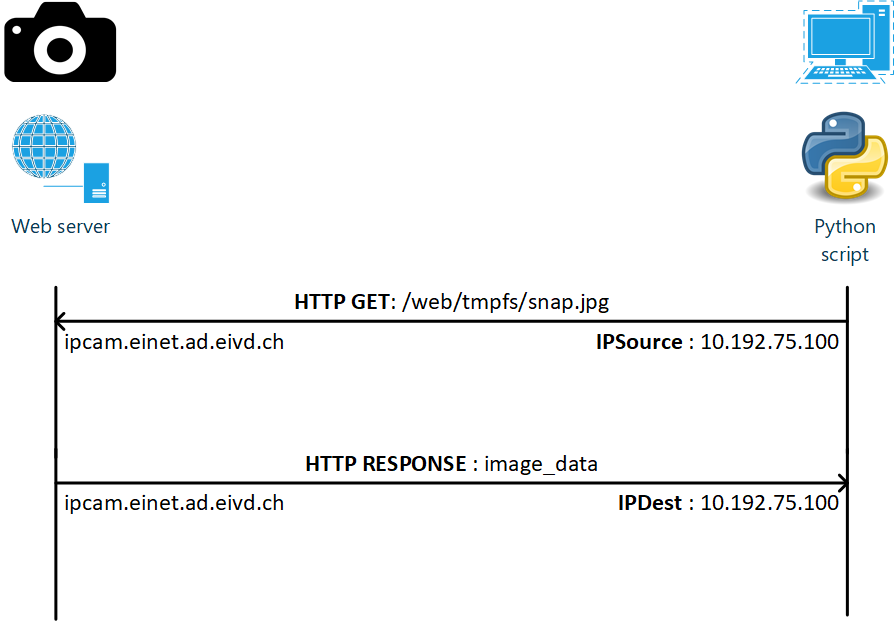
\includegraphics[width=130mm]{img/realisation/cam_request.png}
    \centering
    \caption{Requête d'une image à la caméra \textbf{Wanscam} \textit{HW0029-5}}
    \label{fig:image_request}
\end{figure} 

\subsection{Agent}\label{realisation.capture.agent}
Un agent a été développé, déployé sur la VM. Celui-ci permet de définir un intervalle auquel des images seront demandées à la caméra. Il permet donc de gérer la connexion à celle-ci, mais aussi les pertes de liaisons. A la réception d'une image, il permet de définir une méthode de traitement (décrite en section \ref{conception.traitement} et \ref{realisation.traitement}). 
Il permet aussi de définir, si tel est souhaité, une heure de début et une heure de fin durant lesquelles les requêtes seront effectuées. Lorsqu'on sort de cet intervalle, aucune photo ne sera capturée. Dans notre cas, celui-ci est utilisé afin d'éviter une multitude d'images prises du parking vide aux heures de nuit.

On trouvera au listing \ref{lst:agent} la création en python de celui-ci. Il faut remarquer qu'il n'a pas été souhaité de préciser les constantes \lstinline[columns=fixed]{USERNAME} et \lstinline[columns=fixed]{PASSWORD} pour des raisons de confidentialité. Il est aussi nécessaire de préciser que \lstinline[columns=fixed]{handle_image} est la fonction qui décrit le traitement effectué sur chaque image reçue. Celle-ci sera décrite en section \ref{realisation.traitement}

% spellcheck-language "en"
\begin{lstlisting}[caption={Création d'un agent récupérant les images}, label={lst:agent}] 
CAMERA_HOST = "ipcam.einet.ad.eivd.ch"
IMAGE_REQUEST_MIN_DELTA = 60
IMAGE_REQUEST_START_TIME = time(4, 30) # Start time at  4h30 AM
IMAGE_REQUEST_STOP_TIME = time(23) # Stop time at 11 PM
# [...]

# Creating a camera client
camera = CameraClient(CAMERA_HOST, USERNAME, PASSWORD)
# Creating a agent which requests the camera for an image once every hour
agent = CameraAgent(camera, handle_image, minutes = IMAGE_REQUEST_MIN_DELTA, running_time=(IMAGE_REQUEST_START_TIME, IMAGE_REQUEST_STOP_TIME))
\end{lstlisting}
% spellcheck-language

Ainsi, une image sera demandée toutes les heures, de 4h30 à 11h.

\subsection{Monitoring}
La caméra utilisée fonctionne sur batterie et panneaux solaires. Ainsi, il a semblé important de pouvoir surveiller le bon fonctionnement du système, et d'être averti en cas de malfonctionnement afin de pouvoir agir au plus vite. On pensera notamment à une perte de connexion due à des batteries faibles (par exemple, suite à un manque de soleil sur plusieurs jours consécutifs), ou encore à un câble déconnecté.

\textit{Python} offre un système complet natif de journalisation. Lorsque ce système est utilisé dans les modules créés, il est aisé de traiter des logs, et même d'avertir par mail des erreurs produites. Ce module peut être importé grâce à l'instruction \lstinline[columns=fixed]{import logging}.

Ce système offre plusieurs niveau de log. On les trouvera ci-dessous, du plus critique au moins important\autocite{doc:log}:
\begin{itemize}
    \item \lstinline[columns=fixed]{CRITICAL}
    \item \lstinline[columns=fixed]{ERROR}
    \item \lstinline[columns=fixed]{WARNING}
    \item \lstinline[columns=fixed]{INFO}
    \item \lstinline[columns=fixed]{DEBUG}
    \item \lstinline[columns=fixed]{NOTSET}
\end{itemize}

Ainsi, le niveau de chacun des logs effectués lors de la capture d'image a été défini. Une liste des logs importants concernant ce monitoring est proposée ci-dessous:
\begin{description}
    \item[INFO] Une image a été capturée et bien reçue
    \item[ERROR] La connexion à la caméra a été perdue
    \item[INFO] La caméra n'est toujours pas accessible
    \item[WARNING] La connexion à la caméra a été rétablie
\end{description}

\textit{Python} permet d'écouter les logs émis par un module. Il est aussi possible de définir le niveau d'écoute. Par exemple, il peut être souhaité de capturer tous les logs de niveau \textit{WARNING}. Dans ce cas, tous les logs de ce type seront capturés, ainsi que tous les logs dont le niveau est supérieur (soit plus important). 

Lors de l'arrivée d'un log, un système de \textit{handler} (proposé par \textit{Python}) a été mis en place. On en distinguera 3:
\begin{description}
    \item[Terminal handler] Ecoute les logs à partir du niveau \textit{INFO}. A l'arrivée d'un log, celui-ci est affiché dans la console. Les informations de debug ne sont pas affichées.
    \item[File handler] Ecoute tous les logs. Ainsi, une trace est gardée de tous les logs dans le système de fichier. Ce gestionnaire est de type \lstinline[columns=fixed]{TimedRotatingFileHandler}, qui permet de créer un nouveau fichier de logs par jour. 
    \item[SMTPHandler] Ecoute les logs à partir du niveau \textit{WARNING}. Lors d'une erreur ou d'un avertissement, un mail est envoyé automatiquement.
\end{description}

Ainsi, il est possible d'agir rapidement lors d'une perte de connexion à la caméra. Le log associé étant de type (\textit{ERROR}), un mail est envoyé à l'aide du \textit{SMTPHandler}. Si la caméra est reconnectée (\textit{WARNING}), un mail est aussi reçu.

\section{Traitement des images}\label{realisation.traitement}

La figure \ref{fig:image_process} présente la récupération et le traitement des images qui est effectué.

\begin{figure}[ht]
    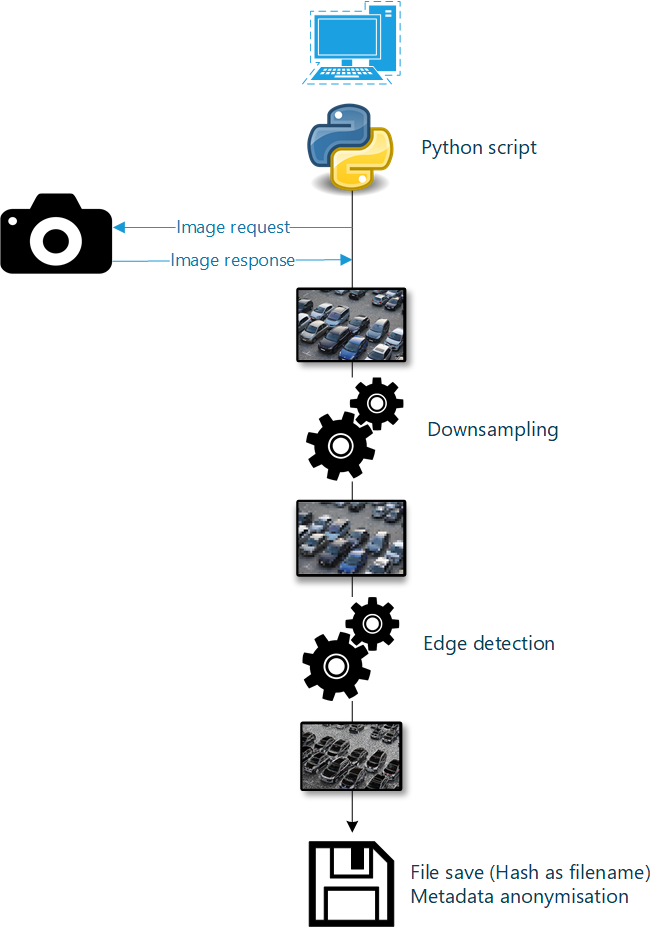
\includegraphics[width=110mm]{img/realisation/image_process.png}
    \centering
    \caption{Requêtes d'images et traitement}
    \label{fig:image_process}
\end{figure} 

Dans un premier temps, un script Python interroge la caméra et récupère une image tel qu'il a été décrit en section \ref{realisation.capture} précédente. Ensuite, l'image est sous-échantillonnée, et les bords détectés. Pour ce faire, \textit{Scikit-image} a été utilisé.

Le code \ref{lst:handling_image} présenté montre la méthode traitant les images entrantes. Celles-ci sont passées en argument de la méthode (\lstinline[columns=fixed]{image_stream}).


% spellcheck-language "en"
\begin{lstlisting}[caption={Traitement des images reçues}, label={lst:handling_image}] 
# Defining what to do when an image is received
def handle_image(image_stream):
    # Converting to a skimage/opencv image (simply a [x, y, 3] numpy array)
    image = io.imread(image_stream)

    # Firstly, downsampling the image
    image = transform.resize(image, IMAGE_OUTPUT_SIZE, mode='reflect', anti_aliasing=True)

    # Secondly, detecting the edges
    image = scharr_hsv(image)

    # Then, we output the image to the folder
    # We use a hash as an ID
    # We could have used a datetime format as a unique filename, but this could results to a lack of privacy
    # Saving it as a bitmap: no decompression to do when loading a lot of file
    # Note: hashing time is negligible
    h = hash(image.data.tobytes())
    filename = IMAGE_FOLDER + hex(h)[-15:] + ".bmp"

    with warnings.catch_warnings(): # used to ignore loss of precision warning
        warnings.simplefilter("ignore")
        io.imsave(filename, image)

    # We then have to reset metadata access and edit time because of privacy issues
    os.utime(filename, (946684800, 946684800))
\end{lstlisting}
% spellcheck-language

La méthode \lstinline[columns=fixed]{_scharr_hsv} utilisée est décrite au listing de code \ref{lst:scharr_filter}. 

Il est possible d'y distinguer la ligne \lstinline[columns=fixed]{@adapt_rgb(hsv_value)}, 

provenant de la librairie \textit{scikit-image}. Elle permet d'adapter le filtre \textit{scharr} présent dans la méthode sur chacun des canaux de l'image.

% spellcheck-language en
\begin{lstlisting}[caption={Détection de bord à l'aide de \textit{scikit-image}}, label={lst:scharr_filter}] 
@adapt_rgb(hsv_value)
def _scharr_hsv(image):
    return filters.scharr(image)
\end{lstlisting}
% spellcheck-language

Dans le cadre de l'anonymisation des données, il a semblé important qu'aucune information concernant les utilisateurs puisse apparaître. C'est pourquoi le nom de l'image est basé sur son hash (fonction de hash fournie par Python. Un hash complexe n'est pas nécessaire). 

L'image est ensuite sauvegardée à un format \textit{bitmap} (\textit{.bmp}), sans pertes de compression. La date et l'heure de création et de modification du fichier sont aussi modifiées pour que les données soient au plus anonymisées.

\section{Traitement du corpus \textit{PKLot}} \label{realisation.dataset}

Les images fournies par \textit{PKLot} sont annotées par place de parc marquée au sol. Cependant, il est possible que certaines voitures ne soient pas stationnées sur l'une de celle-ci. 

Si lors de l'entrainement, l'image segmentée par place de parc est utilisée, cela ne poserait aucun problème. Cependant, dans le cadre de ce projet, les modèles sont entrainés sur l'ensemble de l'image. Ainsi, certaines voitures présentes n'ont pas été annotées comme telles. Si ce \textit{dataset} n'était pas traité, certaines voitures seraient considérés comme étant de l'arrière-plan, et ne seraient pas détectée. 

\begin{figure}[ht]
    
    \begin{subfigure}{\textwidth}
        \centering
        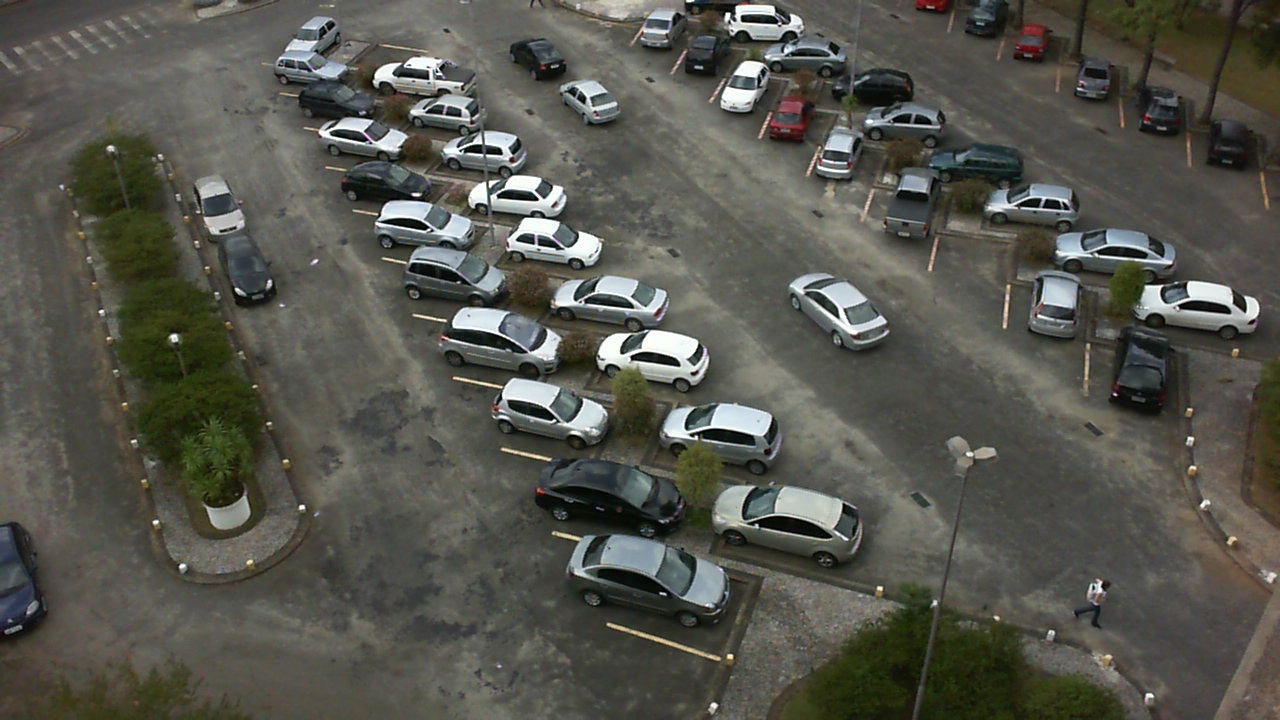
\includegraphics[width=.6\linewidth]{img/realisation/fill_before.jpg}
        \caption{Avant remplissage}
    \end{subfigure}%   

    \bigskip
    \begin{subfigure}{\textwidth}
        \centering
        
\includegraphics[width=.6\linewidth]{img/realisation/fill_mask.png}
        \caption{Masque utilisé}
    \end{subfigure}

    \bigskip
    \begin{subfigure}{\textwidth}
        \centering
        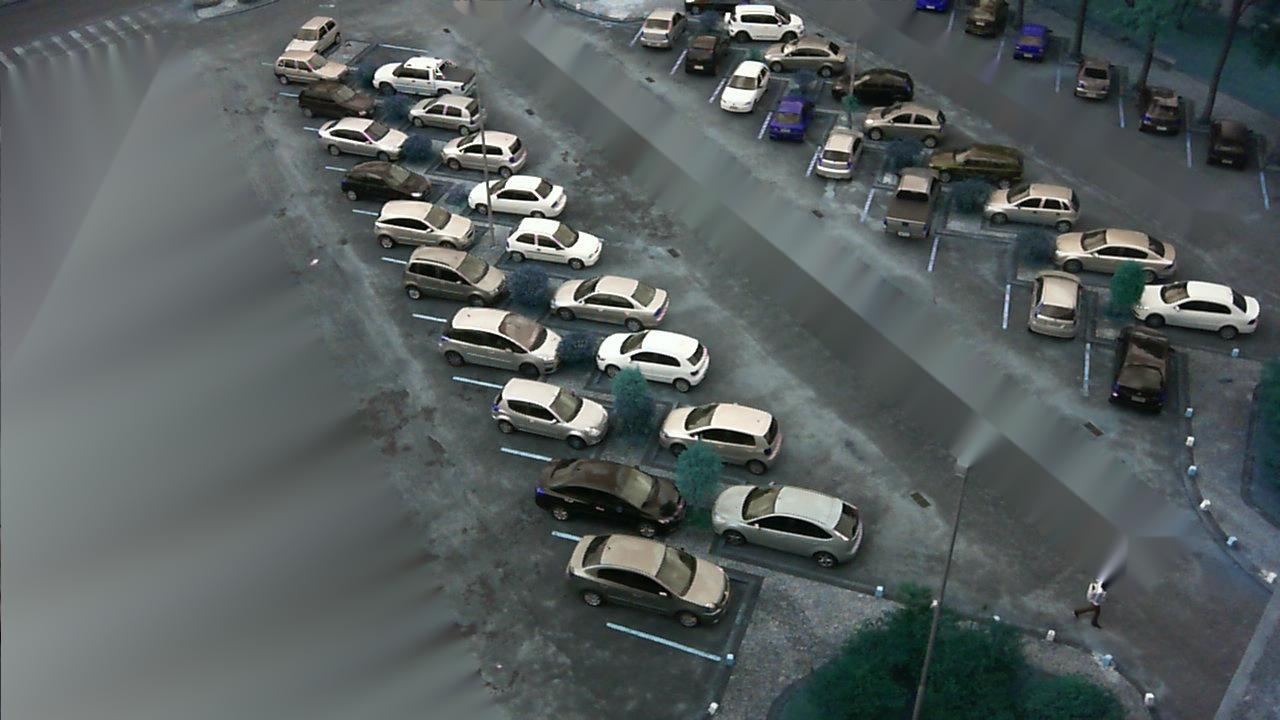
\includegraphics[width=.6\linewidth]{img/realisation/fill_after.jpg}
        \caption{Après remplissage}
    \end{subfigure}

    \caption{Avant-après traitements d'une image du corpus \textit{PKLot}}
    \centering
    \label{fig:image_fill_compare}
\end{figure}

Le corpus \textit{PKLot} est séparé en 3 dossiers différents pour chacune des caméras disponibles. Chaque image a été traitée à l'aide d'une méthode de remplissage, permettant d'effacer certaines régions d'une image\autocite{wiki:inpainting}. Pour ce faire, \textit{OpenCV} a été utilisé. La figure \ref{fig:image_fill_compare} en présente un résultat.

Il faut noter qu'un remplissage de qualité n'est pas nécessaire. En effet, il est avant tout nécessaire d'effacer les voitures présentes qui n'ont pas été annotée comme telles. 

Par la suite, les entrainements qui ont été effectués utilisent l'ensemble de ces images traitées, sans distinction entre les caméras. Cela permet d'augmenter la généralisation des modèles générés.

\section{Mise en place et entrainements des modèles}

\subsection{Machine virtuelle}
Afin d'obtenir de meilleures performances pour l'entrainement des modèles, une machine virtuelle a été créée sur \textit{AWS} \footnote{\textit{AWS}, pour \textit{Amazon Web Service}, fourni un système de IaaS (\textit{Infrastructure as a Service} où il est possible, entre autres, d'instancier des machines virtuelles puissantes). \url{https://aws.amazon.com/}}. Elle fournit aussi des images d'instances spécialisées dans le \textit{Machine learning}, où par exemple \textit{TensorFlow} et \textit{Keras} sont préinstallés\footnote{Les images sont disponibles à l'adresse \url{https://aws.amazon.com/fr/machine-learning/amis/}.}. C'est celle-ci qui a été utilisée. Les corpus d'images nécessaires à l'entrainement y ont été téléchargés et pré-traités à l'aide de scripts \textit{Python} qui ont été développé dans le cadre de ce projet.

\subsection{Format \textit{VOC} \textit{XML}}
Un format courant d'annotations d'images est le format \textit{VOC}, qui permet une certaine interopérabilité. Un exemple en est donnée au code \ref{lst:voc}. Le nom de l'image ainsi que sa taille y est indiqué, Aussi, chaque objet présent dans l'image y est indiqué, ainsi que sa classe et sa \textit{bounding box} associée. Il y a un fichier \textit{VOC} par images.

% spellcheck-language "en"
\begin{lstlisting}[caption={Exemple de fichier \textit{VOC}}, label={lst:voc}, language=XML] 
<annotation>
<filename>2012-11-10_07_12_40.jpg</filename>
<size>
    <width>1280</width>   
    <height>720</height>
    <depth>3</depth>
</size>
<segmented>0</segmented>
<object>
    <name>car</name>
    <bndbox>
        <xmin>669</xmin>
        <ymin>419</ymin>
        <xmax>717</xmax>
        <ymax>475</ymax>
    </bndbox>
</object>
</annotation>
\end{lstlisting}
% spellcheck-language

Les annotations fournies par \textit{PKLot} sont dans un format \textit{XML} qui leurs sont propres. Il a été nécessaire de transcrire ces \textit{XML} au format \textit{VOC}. Pour ce faire, un script \textit{Python} a été utilisé. Celui-ci utilise la librairie \textit{etree} pour \textit{parser} le fichier original, et en créer un nouveau correspondant au format \textit{VOC} voulu. 

\subsection{\textit{Tensorflow Object Detection API}}
Comme précédemment indiqué dans ce rapport, l'API de détection d'objets fournie par \textit{Tensorflow} a été utilisée. Celui-ci n'étant pas inclus dans \textit{TensorFlow}, le \textit{repo}\footnote{On trouvera le repo sur \url{https://github.com/tensorflow/models/tree/master/research/object_detection}} de l'API a été cloné et utilisé. Il a été nécessaire de l'ajouter aux variables d'environnements \textit{Python} afin qu'il soit possible d'importer directement les librairies nécessaires depuis un script \textit{Python}.

Afin d'utiliser un corpus d'entrainement à l'aide de \textit{Tensorflow}, des fichier \textit{.record} doivent être généré. Ceux-ci contiennent les images et leurs annotations. Ils peuvent être aisément créés à partir de fichiers \textit{VOC} à l'aide de la librairie \textit{TensorFlow} et d'un script \textit{Python}. 

Un fichier de configuration (\textit{.config}) est aussi nécessaire. Celui-ci indique où se situe les fichiers \textit{.record}, le modèle pré-entrainé, etc. Par la suite, l'entrainement est exécuté en ligne de commande.

% spellcheck-language "en"
\begin{lstlisting}[caption={Exécution d'un entrainement à l'aide de \textit{Tensorflow Object Detection API}}, label={lst:cmd_train}, numbers=none] 
python /home/ubuntu/tensorflow_models/research/object_detection/train.py \
--logtostderr \
--train_dir=/home/ubuntu/DS/PKLot/tensorflow_ds/training/ \
--pipeline_config_path=/home/ubuntu/TB/GIT/dev/park_python/drafts/object_detection/tensorflow_api_pklot/training.config
\end{lstlisting}
% spellcheck-language

\subsection{\textit{Yolo}}
Une implémentation de \textit{Yolo} a aussi été utilisée. Pour ce faire, il a été nécessaire de télécharger le code source du réseau de neurones open-source \textit{Darknet}\autocite{lib:yolo}, en clonant le \textit{repo} associé.

Une fois celui-ci téléchargé, l'attribut \textit{OPENMP} du fichier \textit{Makefile} a été défini à 1 afin que les entrainements puissent être effectués sur tous les cœurs de la machine disponible. Puis, le code a été compilé à l'aide de la commande \textit{make} linux. Il faut noter que cette commande n'est pas nativement disponible sous Windows.

Dans un second temps, il est nécessaire de préparer les labels pour l'entrainement. Puisque les formats \textit{VOC} ont été créés pour le corpus \textit{PKLot}, un script \textit{Python} fourni par \textit{Darknet} a été utilisé. Les fichiers de configurations nécessaires à l'entrainement sur le \textit{dataset} ont aussi été modifiés. 

\begin{lstlisting}[caption={Exécution d'un entrainement à l'aide de \textit{Yolo}}, label={lst:yolo_train}, numbers=none] 
./darknet detector train cfg/coco.data cfg/yolov3.cfg darknet53.conv.74
\end{lstlisting}
% spellcheck-language


\section{Utilisation du modèle final \textit{Tensorflow}} 
Comme l'indique les tests en section \ref{tests.final} \itnameref{tests.final}, un modèle utilisant l'API de \textit{Tensorflow} a été choisi. 

Une classe, \textit{TensorflowPredictor}, a été créée, basée sur des codes d'exemples disponibles (dont les sources sont précisiées dans le code source). Lors de son instanciation, le chemin vers le modèle qu'on souhaite utiliser est passé en paramètre, ce qui a pour effet de le charger en mémoire. Ensuite, il est possible d'utiliser cet objet afin de prédire le nombre de voitures présentes sur une image. Le script permet aussi une exécution en ligne de commande afin de pouvoir générer les \textit{bounding box} d'une image.

\todo{Préciser la structure du projet, et liens github}



